\documentclass{beamer}

\usepackage[utf8x]{inputenc}
\usepackage[english]{babel}
\usepackage[export]{adjustbox}

\mode<presentation> {
	\usetheme{Berlin}
}

\usebackgroundtemplate {
	
\includegraphics[width=370px, height=270px, trim=0 0 0 -80px]{BackTriangles025.png}
}

\title[High Performance Conference, September 02-06, 2019, Borovets, Bulgaria]{
	Genetic Algorithm Based Formula Generation for Curve Fitting in Time Series Forecasting Implemented as Mobile Distributed Computing
}

\author{Rumen Ketipov, Georgi Kostadinov, Plamen Petrov,\\ Iliyan Zankinski, Todor Balabanov\textsuperscript{0000-0003-3139-069X}}

\date{02-06.IX.2019}

\institute[IICT-BAS, HPC'19] {
	Institute of Information and Communication Technologies \\ 
	Bulgarian Academy of Sciences \\
	\medskip
	\textit{todorb@iinf.bas.bg}
}

\addtobeamertemplate{navigation symbols}{}{
    \usebeamerfont{footline}
    \usebeamercolor[fg]{footline}
    \hspace{1em}
    \insertframenumber/\inserttotalframenumber
}

\begin{document}

\begin{frame}
\titlepage
\end{frame}

\begin{frame}
\frametitle{Agenda}
\tableofcontents
\end{frame}

\section{Introduction}

\begin{frame}
\center \huge{Introduction}
\end{frame}

\subsection{Time Series}

\begin{frame}
\frametitle{Financial Time Series}
\begin{itemize}
	\item Area of high researchers interest from many decades
	\item Having an accurate forecast in the financial world is crucial for many important decision makings
	\item Time series are ordered measurements of particular variable done in a temporal manner
	\begin{itemize}
		\item In the most cases values are measured on equal intervals
		\item But it is not a mandatory 
	\end{itemize}
\end{itemize}
\end{frame}

\begin{frame}
\frametitle{Time Series Forecasting}
\begin{itemize}
	\item It is applicable in processes with clear repetition pattern
	\item Measurements done in a temporal order are presented as points in a two-dimensional space
	\item Visually these points are connected with straight lines (simplified form of linear interpolation for the values between two neighboring measurements)
	\item In such two-dimensional space many different curves can be proposed for some generalization of the data nature (curve fitting problem)
	\begin{itemize}
		\item Linear regression can be used for trend estimation
		\item Lagrange polynomial as more complex generalization
	\end{itemize}
\end{itemize}
{\color{red} Infinite number of curves can satisfy the condition to pass across finite number of points in two-dimensional space}
\end{frame}

\subsection{Evolutionary Computing}

\begin{frame}
\frametitle{Genetic Algorithms}
\begin{itemize}
	\item Meta-heuristic for global optimization inspired by the natural processes in the biological evolution
	\item Population based algorithms sub-class of the evolutionary algorithms
	\begin{itemize}
		\item Each individual is a vector into the solutions space
	\end{itemize}
	\item Based on three general operations - selection, crossover and mutation
\end{itemize}
\end{frame}

\begin{frame}
\frametitle{Optimization Remarks}
\begin{itemize}
	\item Proper encoding of the individuals (expression tree encoding in this study)
	\item Selection of parents (tournament selection in this study)
	\begin{itemize}
		\item With elitism rule applied
	\end{itemize}
	\item Crossover for exploration capabilities (single cut point in this study)
	\item Mutation for exploitation capabilities (random change of mathematical operation and random change of the operand in this study)
	\item Fitness value evaluation (curve fitting closeness in this study)
\end{itemize}
\end{frame}

\subsection{Distributed Computing}

\begin{frame}
\frametitle{Distribution of Computations}
\begin{itemize}
	\item A computational organization in a system where components are located on different networked computers
	\item Computers communicates and coordinates their activities by passing messages between each other
	\item It is remarkable with:
	\begin{itemize}
		\item Concurrency of components
		\item Lack of a global clock
		\item Independent failure of components
	\end{itemize}
\end{itemize}
\end{frame}

\begin{frame}
\frametitle{How Distributed Computing is Done}
\begin{itemize}
	\item A problem is divided into many tasks
	\item Each task is solved by one or more computers
	\item Computers communicate with each other via message passing
\end{itemize}
{\color{red} Distributed computing is generally used for solving a large computational problems}
\end{frame}

\section{Proposed Solution}

\begin{frame}
\center \huge{Proposed Solution}
\end{frame}

\subsection{Donated Distributed Computing}

\begin{frame}
\frametitle{Donated Calculating Power}
\begin{itemize}
	\item Users donate their computational resources
	\item In most cases computations are organized as screen-saver applications
	\item It is mainly used for low budget projects usually in society help
\end{itemize}
\end{frame}

\begin{frame}
\frametitle{Mobile Distributed Computing}
\begin{itemize}
	\item Modern mobile devices have significant computation capabilities
	\item Most of the mobile devices are operating 24x7
	\item Active wallpaper is used instead screen-saver
\end{itemize}
Widgets are also an option, which can extend the idea to human-computer based distributed computing
\end{frame}

\subsection{Expressions Evaluation}

\begin{frame}
\frametitle{Structures and Operators}
\begin{itemize}
	\item Simple text representation of mathematical expressions
	\item Single point cut crossover
	\item Random change of mathematical operator mutation
	\item Random change of mathematical operand mutation
\end{itemize}
\end{frame}

\begin{frame}
\frametitle{Optimization Procedure}
\small
begin \\
~  t = 0; \\
~  initialize P(t); \\
~  evaluate structures in P(t); \\
~  while termination condition not satisfied do \\
~  begin \\
~~    t = t + 1; \\
~~    select\_repro C(t) from P(t-1); \\
~~    recombine and mutate structures in C(t) \\
~~    forming C'(t); \\
~~    evaluate structures in C'(t); \\
~~    select\_replace P(t) from C'(t) and P(t-1); \\
~  end \\
end \\
\end{frame}

\begin{frame}
\frametitle{Solutions Fitness}
\begin{itemize}
	\item Invalid formulas are ignored
	\item Calculation of the valid formula 
	\item Fitness is the mean square of the error with the real life values
\end{itemize}
\end{frame}

\subsection{Client-Server Communication}

\begin{frame}
\frametitle{Keeping Solutions}
\begin{itemize}
	\item Best found local solutions are reported to the remote server
	\item On the remote server global population is kept
	\item When new mobile client is connected subset of the global population is sent as new local population
\end{itemize}
\end{frame}

\section{Experiments and Results}

\begin{frame}
\center \huge{Experiments and Results}
\end{frame}

\subsection{Experimental Platform}

\begin{frame}
\frametitle{Software Solution}
\begin{itemize}
	\item Android mobile application on the client side
	\item Apache Commons Genetic Algorithms Framework is used for evolutionary optimization
	\item Mathematical expressions are presented and evaluated with mXparser library
	\item PHP/MySQL custom solution is used on the server side
\end{itemize}
\end{frame}

\subsection{Optimization Parameters}

\begin{frame}
\frametitle{Genetic Algorithm Parameters}
\begin{table}
	\begin{tabular}{p{5.4cm}p{4.4cm}}
		\hline
		\textbf{Parameter} & \textbf{Value} \\
		\hline
		generation gap & 0.97 \\
		crossover rate & 0.95 \\
		mutation rate & 0.03 \\
		maximum generations & 100 \\
		number of individuals & 37 \\
		number of variables & floating \\
		inserted rate & 100 \% \\
		\hline
	\end{tabular}
\end{table}
\end{frame}

\begin{frame}
\frametitle{EUR/USD Rate for Two Months}
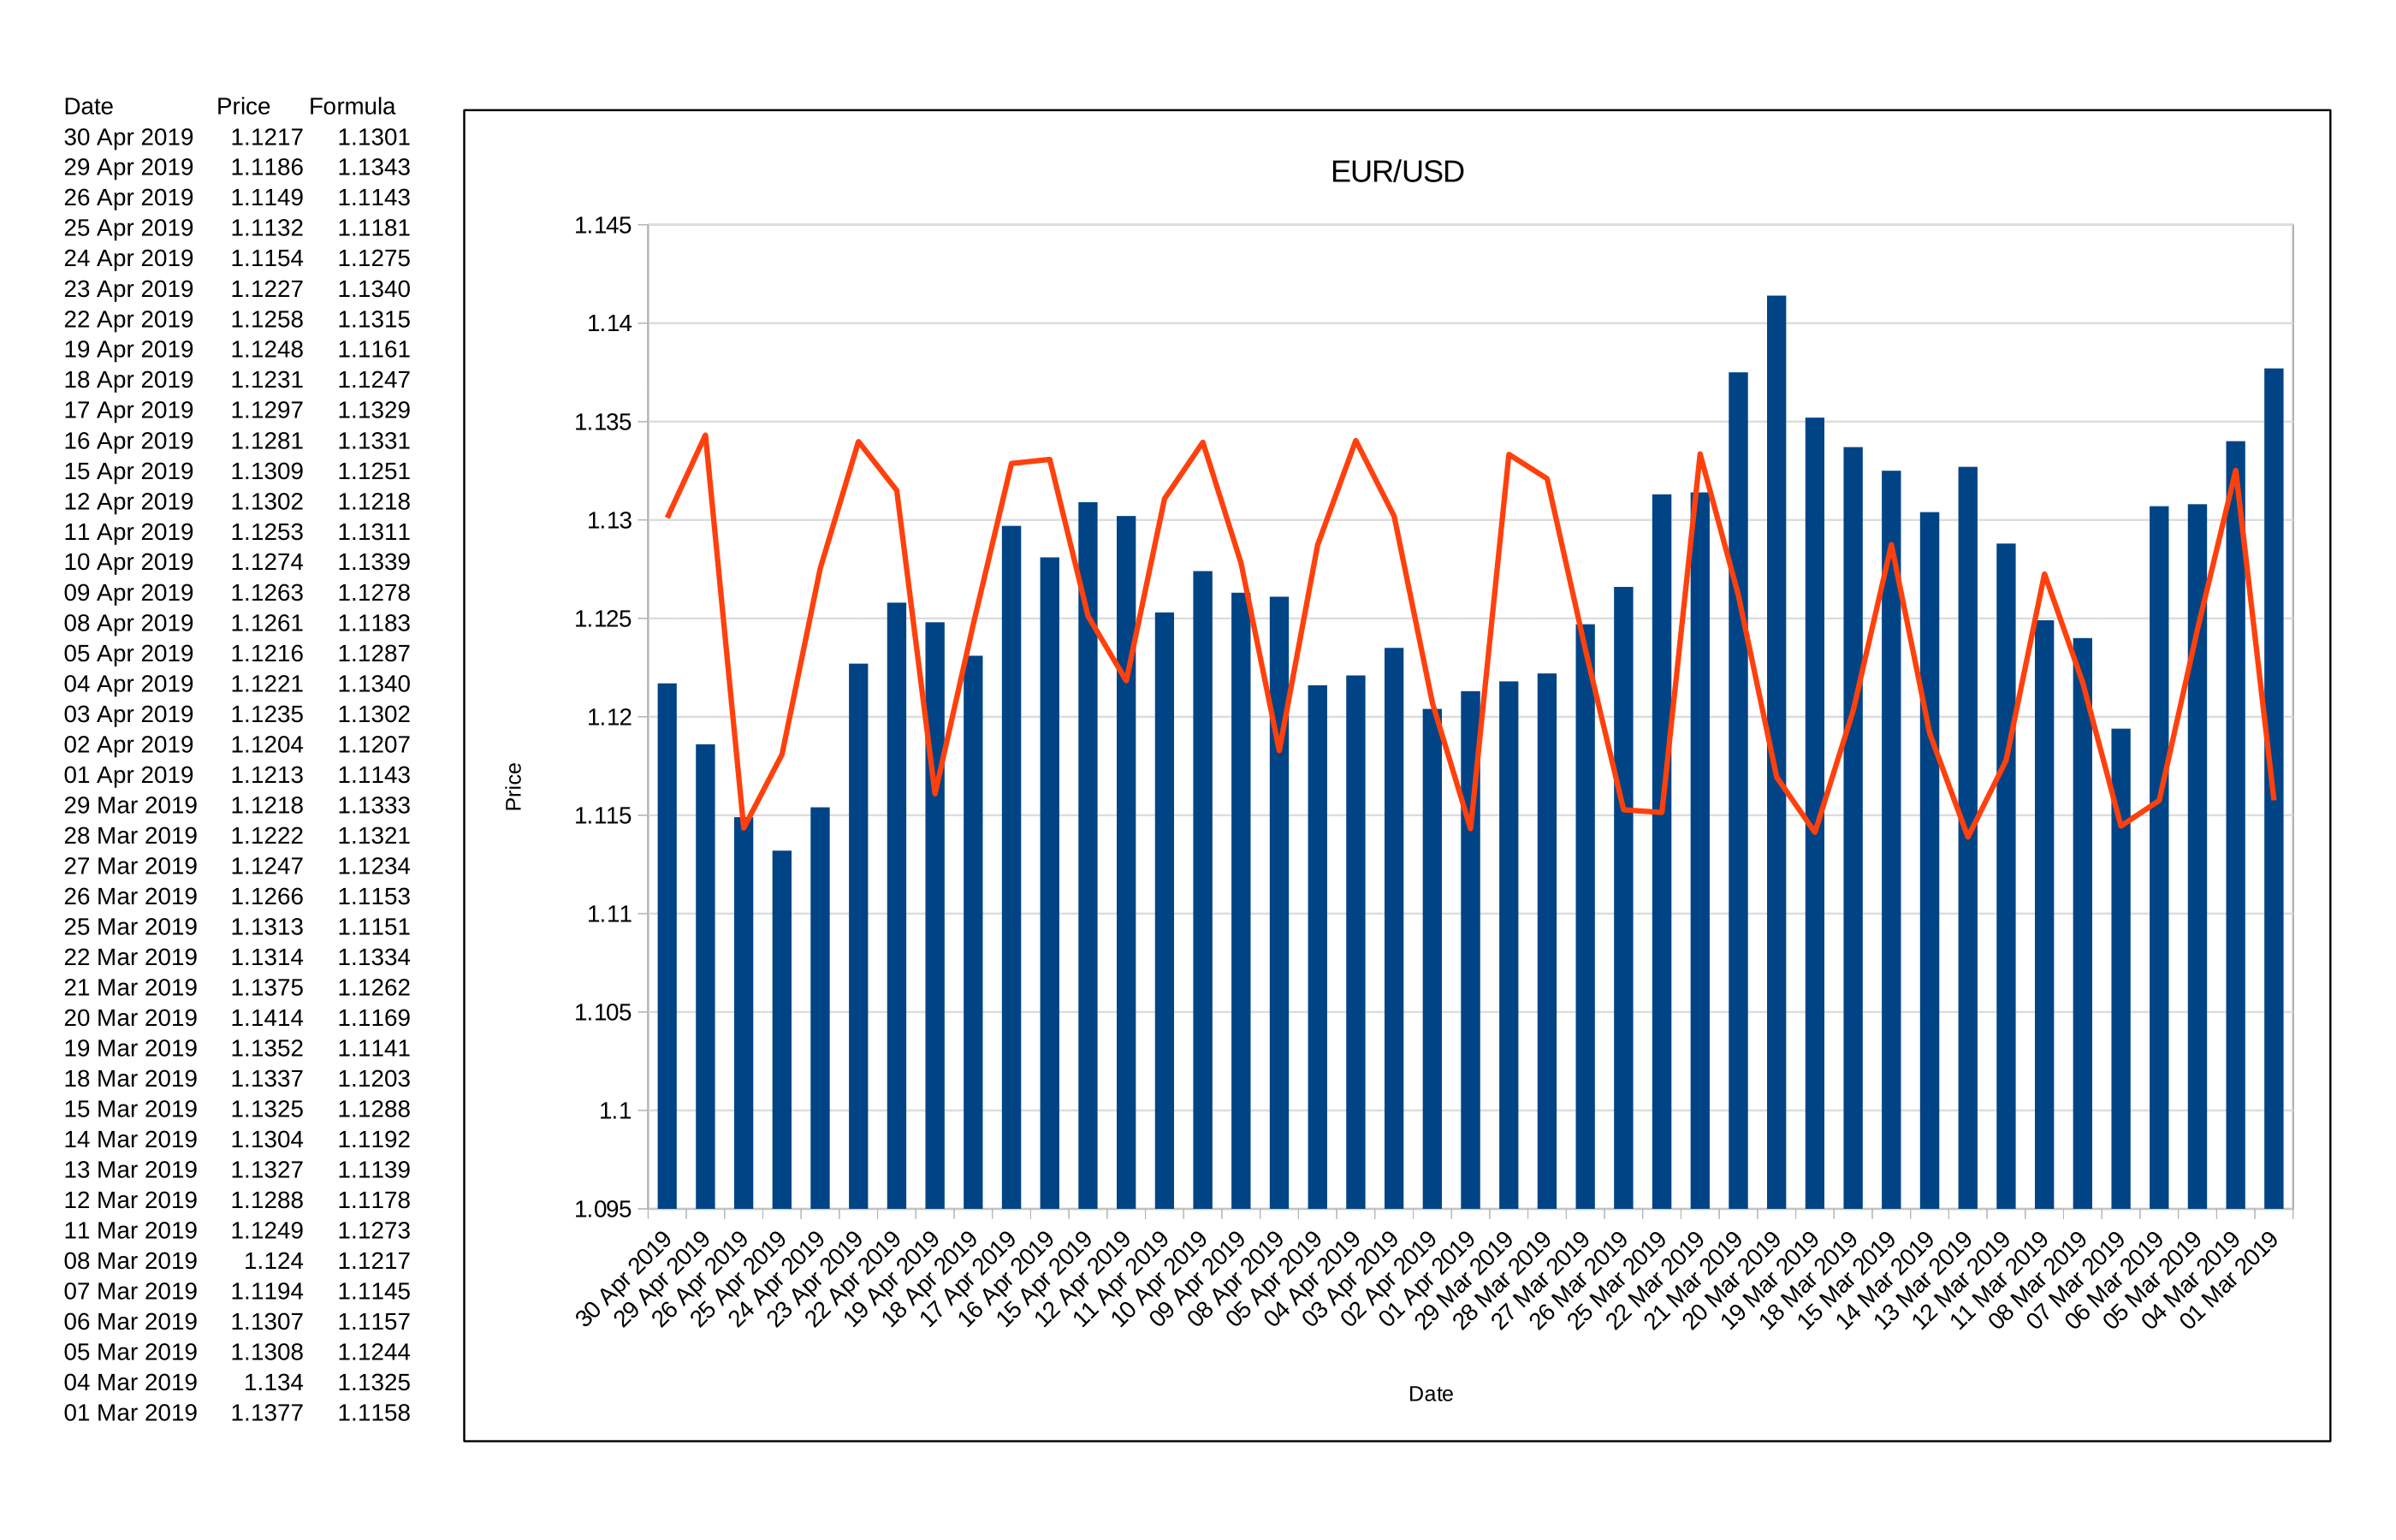
\includegraphics[scale=0.09]{fig01.png}
\end{frame}

\section{Conclusions}

\begin{frame}
\center \huge{Conclusions}
\end{frame}

\subsection{Advantages and Disadvantages}

\begin{frame}
\frametitle{Advantages}
\begin{itemize}
	\item Expressions evolution with genetic algorithms can be a promising approach for financial time series forecasting
	\item The nature of genetic algorithms allows extremely high degree of parallel computations
	\item Many sub-optimal solutions can be provided
\end{itemize}
\end{frame}

\begin{frame}
\frametitle{Disadvantages}
\begin{itemize}
	\item Formulas generation is time consuming process
	\item Financial time series are not constant they are evolving
	\begin{itemize}
		\item Need of recalculation with the time passing
	\end{itemize}
\end{itemize}
\end{frame}

\begin{frame}
\frametitle{Future Research}
\begin{itemize}
	\item Genetic algorithms to be combined with other optimization methods like:
	\begin{itemize}
		\item Particle swarm optimization
		\item Simulated annealing
		\item Tabu search
	\end{itemize}
\end{itemize}
\end{frame}

\subsection{Discussion}

\begin{frame}
\frametitle{Questions and Answers}
\center \huge{Thank you for the attention!}
\end{frame}

\end{document}
